\begin{center}
    \section*{\fontsize{20}{20}\selectfont Chapter 3}
\end{center}

\vspace{6mm}

\section{Research Methodology}

This chapter presents the methodology and architecture of the proposed EHealth system. The platform integrates mobile healthcare services, AI-assisted triage and clinical documentation, WebRTC consultation, relational data storage, and blockchain-based prescription verification.

The methodology focuses on four primary objectives:

\begin{itemize}
    \setlength{\itemsep}{1pt}
    \item AI-based symptom triage using structured LLM output.
    \item Automated speech-to-structured clinical report generation.
    \item Secure video consultation and healthcare service management.
    \item Tamper-evident prescription verification using Polygon PoS.
\end{itemize}

\subsection{Proposed Framework}

The EHealth platform is divided into five functional zones, as illustrated in Figure~\ref{fig:sysarch}.

\begin{figure}[htbp]
\centering
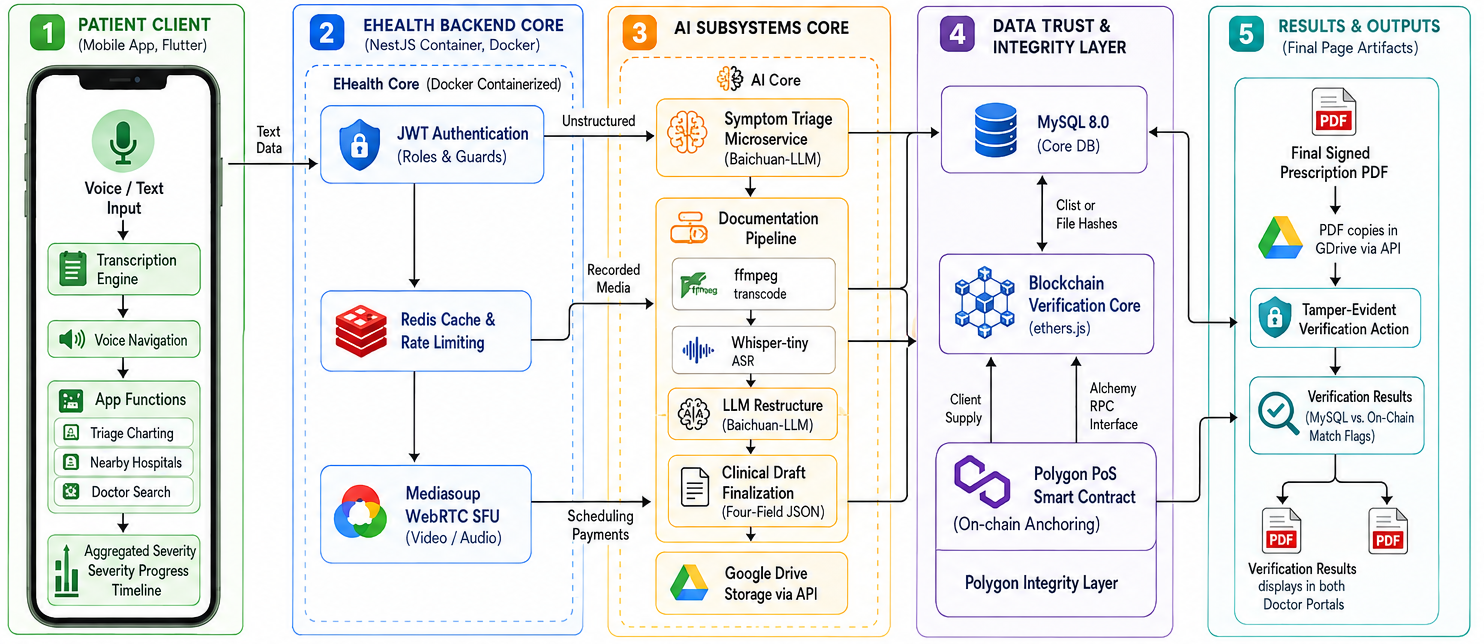
\includegraphics[width=\linewidth]{image/system_architecture_report.png}
\caption{EHealth System Architecture: Five-zone end-to-end clinical workflow.}
\label{fig:sysarch}
\end{figure}

\noindent\textbf{Zone 1 -- Patient Client.}
The Flutter mobile application accepts voice and text input. Voice input is transcribed before transmission, while text is sent directly to the backend. The application also provides triage history, severity trends, nearby hospital information, and doctor search.

\noindent\textbf{Zone 2 -- EHealth Backend Core.}
The NestJS backend manages authentication, scheduling, payment, and consultation services. JWT guards enforce role-based access, Redis provides caching and rate limiting, and Mediasoup SFU supports WebRTC audio/video sessions.

\noindent\textbf{Zone 3 -- AI Subsystems Core.}
Two AI pipelines are implemented. The triage service uses Baichuan-M2-32B to classify symptoms into structured urgency levels. The documentation pipeline converts recorded consultation media to WAV using FFmpeg, transcribes it using Xenova/whisper-tiny, and restructures the transcript into clinical fields using Baichuan-M2-32B. The resulting report is generated as a PDF and stored through the Google Drive API.

\noindent\textbf{Zone 4 -- Data Trust and Integrity.}
MySQL 8.0 stores application data. Final prescription PDFs are hashed and anchored to a Polygon PoS smart contract through ethers.js and the Alchemy RPC interface. Verification independently checks database and blockchain hashes.

\noindent\textbf{Zone 5 -- Results and Outputs.}
The system provides signed prescription PDFs, Google Drive links, and verification results to both doctor and patient interfaces.

\cleardoublepage

\subsection{Software Project Requirements}

Since EHealth is a software engineering project, the evaluation focuses on functional requirements, quality attributes, and internally constructed test data.

\subsubsection{Functional Requirements}


\vspace{3mm}
{
\renewcommand{\arraystretch}{1.3}
\begin{xltabular}{\textwidth}{|>{\centering\arraybackslash}p{1.0cm}|>{\raggedright\arraybackslash}p{3.0cm}|>{\raggedright\arraybackslash}X|>{\centering\arraybackslash}p{1.5cm}|}

% 1. FIRST HEAD (First page header)
\hline
\textbf{ID} & \textbf{Module} & \textbf{Requirement} & \textbf{Priority} \\
\hline
\endfirsthead

% 2. HEAD (Continuation pages header)
\hline
\textbf{ID} & \textbf{Module} & \textbf{Requirement} & \textbf{Priority} \\
\hline
\endhead


% 4. LAST FOOT (only appears once, at the very end of the table)
\hline
\caption{Key Functional Requirements} \label{tab:funcreq} \\
\endlastfoot


% 5. TABLE DATA
FR-01 & Authentication & JWT-based Patient, Doctor, and Admin access control. & High \\
\hline
FR-02 & Triage & Classify symptoms as HIGH, MEDIUM, or LOW with structured JSON output. & High \\
\hline
FR-03 & Scheduling \& Payment & Support consultation booking and SSLCommerz payment. & High \\
\hline
FR-04 & Video Conference & Establish WebRTC sessions through Mediasoup SFU. & High \\
\hline
FR-05 & Documentation & Transcribe consultation audio and generate structured clinical reports. & High \\
\hline
FR-06 & Storage & Upload generated reports to Google Drive and link them to patient records. & Medium \\
\hline
FR-07 & Prescription & Generate and digitally sign prescription PDFs. & High \\
\hline
FR-08 & Blockchain & Store prescription hashes on Polygon PoS. & High \\
\hline
FR-09 & Verification & Independently verify database and blockchain hashes. & High \\
\hline
FR-10 & Mobile App & Display triage history, severity trends, hospitals, and doctors. & Medium \\
\hline

\end{xltabular}
}

\vspace{5mm}

\subsubsection{Non-Functional Requirements}
\vspace{3mm}
{
\renewcommand{\arraystretch}{1.3}
\begin{xltabular}{\textwidth}{|>{\centering\arraybackslash}p{1.2cm}|>{\raggedright\arraybackslash}p{2.5cm}|>{\raggedright\arraybackslash}X|>{\raggedright\arraybackslash}p{2.8cm}|}

% 1. FIRST HEAD (First page header)
\hline
\textbf{ID} & \textbf{Attribute} & \textbf{Requirement} & \textbf{Target} \\
\hline
\endfirsthead

% 2. HEAD (Continuation pages header)
\hline
\textbf{ID} & \textbf{Attribute} & \textbf{Requirement} & \textbf{Target} \\
\hline
\endhead


% 4. LAST FOOT (only appears once, at the very end of the table)
\hline
\caption{Non-Functional Requirements} \label{tab:nonfuncreq} \\
\endlastfoot


% 5. TABLE DATA
NFR-01 & Performance & Triage response latency. & $\le$ 4 s p95 \\
\hline
NFR-02 & Performance & 10-minute consultation documentation pipeline. & $\le$ 3 min \\
\hline
NFR-03 & Privacy & Audio and transcripts remain within the server environment. & No third-party ASR \\
\hline
NFR-04 & Cost & Blockchain anchoring cost. & $\le$ \$0.01/write \\
\hline
NFR-05 & Reliability & WebRTC session packet-loss tolerance. & $\le$ 5\% PLR \\
\hline
NFR-06 & Security & JWT validation and byte-exact hash verification. & Guard + parity test \\
\hline
NFR-07 & Portability & Containerized deployment on Linux. & Docker Compose \\
\hline

\end{xltabular}
}
\vspace{5mm}

\subsubsection{Internal Evaluation Data}
\vspace{3mm}
{
\renewcommand{\arraystretch}{1.3}
\begin{xltabular}{\textwidth}{|>{\raggedright\arraybackslash}p{4.2cm}|>{\centering\arraybackslash}p{1.8cm}|>{\raggedright\arraybackslash}X|}

% 1. FIRST HEAD (First page header)
\hline
\textbf{Dataset} & \textbf{Size} & \textbf{Purpose} \\
\hline
\endfirsthead

% 2. HEAD (Continuation pages header)
\hline
\textbf{Dataset} & \textbf{Size} & \textbf{Purpose} \\
\hline
\endhead


% 4. LAST FOOT (only appears once, at the very end of the table)
\hline
\caption{Internal Evaluation Data} \label{tab:datasets} \\
\endlastfoot


% 5. TABLE DATA
Triage Symptom Set & 200 cases & Evaluate urgency classification accuracy. \\
\hline
Doctor--Patient Dialogues & 50 dialogues & Evaluate ASR WER and clinical extraction quality. \\
\hline
Prescription PDF Set & 30 files & Measure blockchain transaction cost and verification behavior. \\
\hline

\end{xltabular}
}

\vspace{5mm}

\subsection{Algorithm and Model Analysis}

\subsubsection{Constrained LLM Triage}

The triage service receives unstructured patient symptom text and uses the Baichuan-M2-32B model to generate a structured response. A schema-constrained prompt requires three fields:

\begin{itemize}
    \setlength{\itemsep}{1pt}
    \item \texttt{urgencyLevel}: HIGH, MEDIUM, or LOW;
    \item \texttt{matchedSymptoms}: normalized symptom list;
    \item \texttt{triageRationale}: short classification explanation.
\end{itemize}

The model temperature is set to 0.2 to reduce output variability. The backend validates the JSON response before returning it to the client. Invalid responses are replaced with a structured fallback. Redis caches normalized repeated inputs for 30 minutes to reduce redundant LLM requests.

\subsubsection{Speech-to-Report Documentation Pipeline}

The documentation pipeline converts recorded doctor--patient consultations into structured clinical reports. Figure~\ref{fig:speech2report} illustrates the process.

\begin{figure}[htbp]
\centering
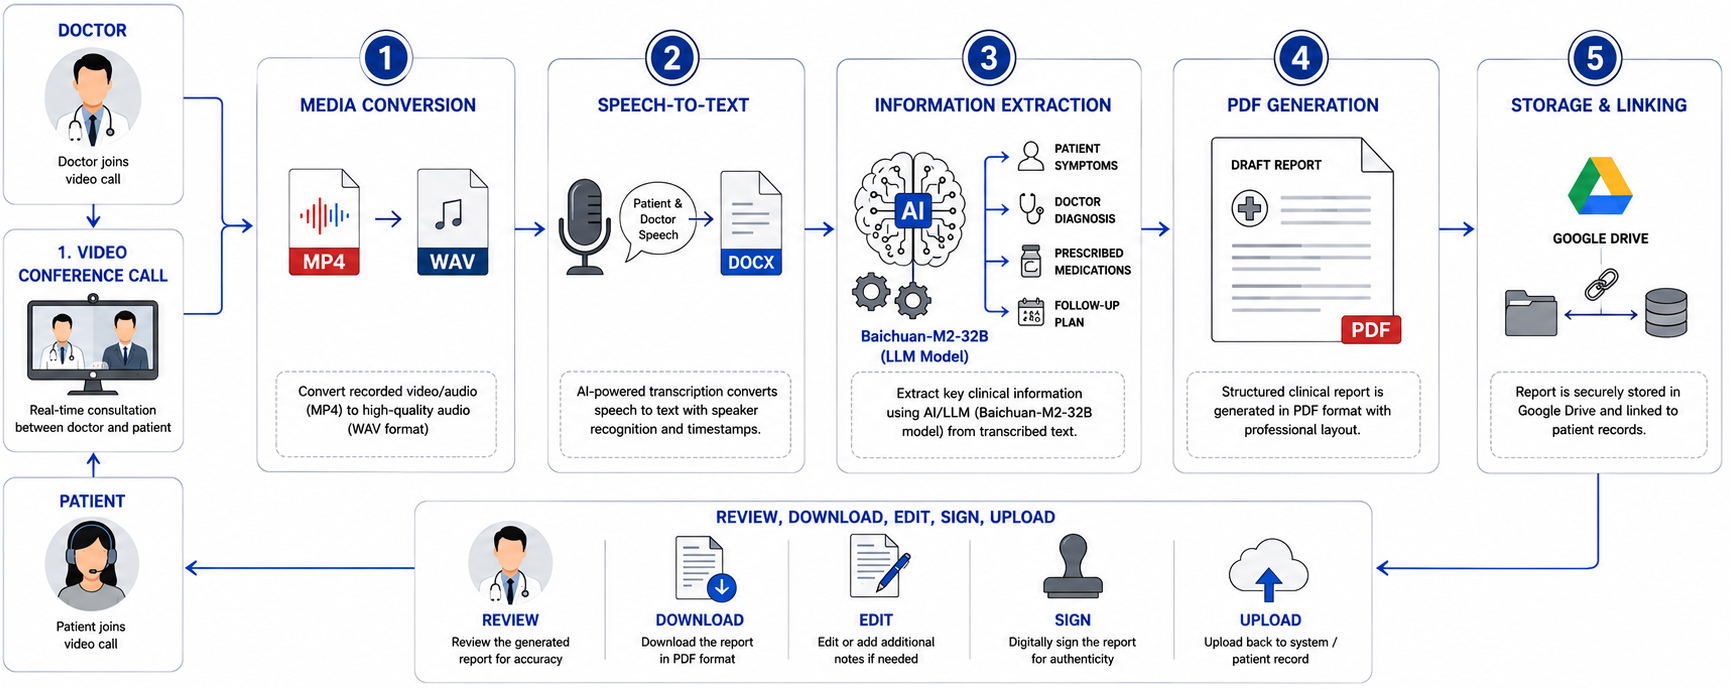
\includegraphics[width=\linewidth]{image/speech_to_report_final.png}
\caption{Speech-to-Report Documentation Pipeline.}
\label{fig:speech2report}
\end{figure}

The pipeline contains five stages:

\begin{enumerate}
    \setlength{\itemsep}{1pt}
    
    \item \textbf{Media Conversion:} FFmpeg converts MP4/WebM recordings into 16\,kHz mono WAV audio.
    
    \item \textbf{Speech-to-Text:} Xenova/whisper-tiny running through ONNX produces the consultation transcript.
    
    \item \textbf{Information Extraction:} Baichuan-M2-32B converts the transcript into four structured fields:
    \texttt{patientSymptoms},
    \texttt{doctorDiagnosis},
    \texttt{prescribedMedications}, and
    \texttt{followUpPlan}.
    
    \item \textbf{PDF Generation:} The structured JSON is rendered as a clinical report for doctor review and signing.
    
    \item \textbf{Storage:} The finalized PDF is uploaded through the Google Drive API, and its link is associated with the consultation record.
\end{enumerate}

\subsubsection{Blockchain Prescription Verification}

Prescription integrity is protected through a dual-state verification mechanism using MySQL and Polygon PoS. Figure~\ref{fig:blockchain} presents the verification flow.

\begin{figure}[htbp]
\centering
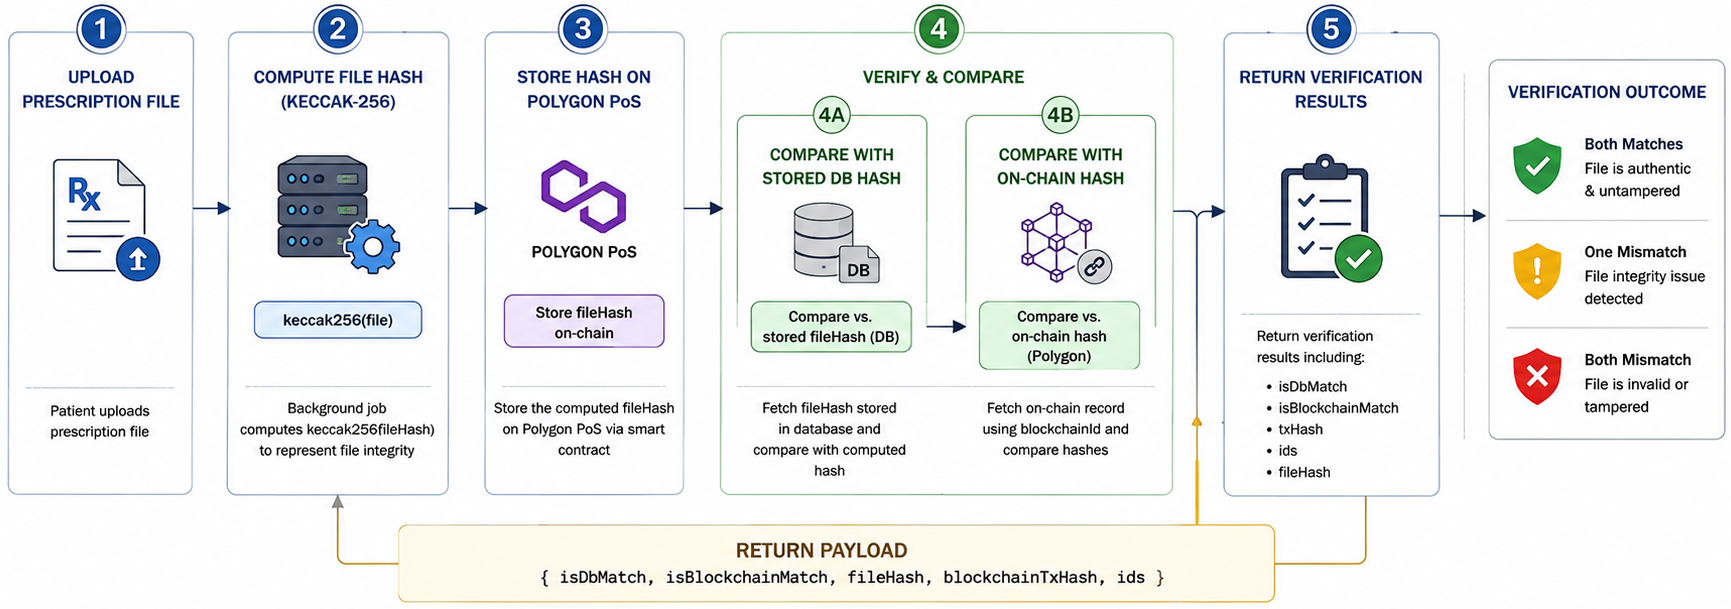
\includegraphics[width=\linewidth]{image/blockchain_polygon_pos_verification_flow_final.png}
\caption{Polygon PoS Prescription Verification Flow.}
\label{fig:blockchain}
\end{figure}

\noindent\textbf{Write Phase:}

\begin{enumerate}
    \setlength{\itemsep}{1pt}
    \item The finalized prescription is hashed using SHA-256 followed by \texttt{keccak256}.
    \item The resulting \texttt{fileHash} is submitted to the Polygon PoS smart contract through ethers.js and Alchemy RPC.
    \item The \texttt{fileHash} and \texttt{blockchainTxHash} are stored with the prescription record.
\end{enumerate}

\noindent\textbf{Verification Phase:}

\begin{enumerate}
    \setlength{\itemsep}{1pt}
    \item The patient uploads a prescription PDF.
    \item The backend recomputes its hash.
    \item The computed hash is independently compared with the MySQL and on-chain hashes.
    \item The system returns:
    \texttt{isDbMatch},
    \texttt{isBlockchainMatch},
    \texttt{fileHash},
    \texttt{blockchainTxHash}, and
    \texttt{ids}.
\end{enumerate}

This dual comparison provides stronger tamper evidence than a single database check. A database mismatch and blockchain mismatch can be reported independently.

\subsection{Explanation of Core Backend Modules}

The backend follows a modular NestJS architecture. Each module separates its controller, service, and DTO responsibilities.

\begin{itemize}
    \setlength{\itemsep}{1pt}

    \item \textbf{Auth Module:} Registration, login, JWT issuance, and role guards.

    \item \textbf{Triage Module:} Input validation, Redis caching, LLM execution, JSON validation, and result storage.

    \item \textbf{Doctor Module:} Doctor profiles, schedules, consultation slots, and fees.

    \item \textbf{Consultation Module:} Payment verification, Mediasoup room management, consultation lifecycle, and pipeline dispatch.

    \item \textbf{Transcription Service:} Audio normalization with FFmpeg and Whisper-based transcription.

    \item \textbf{Consultation Formatter Service:} Baichuan-M2-32B clinical information extraction and structured output validation.

    \item \textbf{Pdf Service:} Clinical PDF generation and storage integration.

    \item \textbf{Prescription Module:} Prescription creation and doctor signature workflow.

    \item \textbf{Blockchain Service:} Hash generation, Polygon transactions, transaction storage, and dual-state verification.
\end{itemize}

\subsection*{Summary}

This chapter presented the methodology of the proposed EHealth platform. The system combines a Flutter client, NestJS backend, AI-based triage and documentation pipelines, MySQL storage, WebRTC consultation, and Polygon PoS prescription verification.

The methodology defines the system architecture, key functional and non-functional requirements, internal evaluation data, AI processing pipeline, blockchain verification process, and backend module structure. Together, these components provide an integrated framework for intelligent clinical support, automated documentation, and tamper-evident prescription verification.